% Options for packages loaded elsewhere
\PassOptionsToPackage{unicode}{hyperref}
\PassOptionsToPackage{hyphens}{url}
%
\documentclass[
]{book}
\usepackage{amsmath,amssymb}
\usepackage{lmodern}
\usepackage{iftex}
\ifPDFTeX
  \usepackage[T1]{fontenc}
  \usepackage[utf8]{inputenc}
  \usepackage{textcomp} % provide euro and other symbols
\else % if luatex or xetex
  \usepackage{unicode-math}
  \defaultfontfeatures{Scale=MatchLowercase}
  \defaultfontfeatures[\rmfamily]{Ligatures=TeX,Scale=1}
\fi
% Use upquote if available, for straight quotes in verbatim environments
\IfFileExists{upquote.sty}{\usepackage{upquote}}{}
\IfFileExists{microtype.sty}{% use microtype if available
  \usepackage[]{microtype}
  \UseMicrotypeSet[protrusion]{basicmath} % disable protrusion for tt fonts
}{}
\makeatletter
\@ifundefined{KOMAClassName}{% if non-KOMA class
  \IfFileExists{parskip.sty}{%
    \usepackage{parskip}
  }{% else
    \setlength{\parindent}{0pt}
    \setlength{\parskip}{6pt plus 2pt minus 1pt}}
}{% if KOMA class
  \KOMAoptions{parskip=half}}
\makeatother
\usepackage{xcolor}
\usepackage{longtable,booktabs,array}
\usepackage{calc} % for calculating minipage widths
% Correct order of tables after \paragraph or \subparagraph
\usepackage{etoolbox}
\makeatletter
\patchcmd\longtable{\par}{\if@noskipsec\mbox{}\fi\par}{}{}
\makeatother
% Allow footnotes in longtable head/foot
\IfFileExists{footnotehyper.sty}{\usepackage{footnotehyper}}{\usepackage{footnote}}
\makesavenoteenv{longtable}
\usepackage{graphicx}
\makeatletter
\def\maxwidth{\ifdim\Gin@nat@width>\linewidth\linewidth\else\Gin@nat@width\fi}
\def\maxheight{\ifdim\Gin@nat@height>\textheight\textheight\else\Gin@nat@height\fi}
\makeatother
% Scale images if necessary, so that they will not overflow the page
% margins by default, and it is still possible to overwrite the defaults
% using explicit options in \includegraphics[width, height, ...]{}
\setkeys{Gin}{width=\maxwidth,height=\maxheight,keepaspectratio}
% Set default figure placement to htbp
\makeatletter
\def\fps@figure{htbp}
\makeatother
\setlength{\emergencystretch}{3em} % prevent overfull lines
\providecommand{\tightlist}{%
  \setlength{\itemsep}{0pt}\setlength{\parskip}{0pt}}
\setcounter{secnumdepth}{5}
\usepackage{booktabs}
\usepackage{amsthm, amsmath, amssymb}
\usepackage{makeidx}
\makeindex
\makeatletter
\def\thm@space@setup{%
  \thm@preskip=8pt plus 2pt minus 4pt
  \thm@postskip=\thm@preskip
}
\makeatother
\ifLuaTeX
  \usepackage{selnolig}  % disable illegal ligatures
\fi
\usepackage[]{natbib}
\bibliographystyle{apalike}
\IfFileExists{bookmark.sty}{\usepackage{bookmark}}{\usepackage{hyperref}}
\IfFileExists{xurl.sty}{\usepackage{xurl}}{} % add URL line breaks if available
\urlstyle{same} % disable monospaced font for URLs
\hypersetup{
  pdftitle={Lecture Note on Terwilliger Algebra},
  pdfauthor={P. Terwilliger, edited by H. Suzuki},
  hidelinks,
  pdfcreator={LaTeX via pandoc}}

\title{Lecture Note on Terwilliger Algebra}
\author{P. Terwilliger, edited by H. Suzuki}
\date{2022-11-17}

\usepackage{amsthm}
\newtheorem{theorem}{Theorem}[chapter]
\newtheorem{lemma}{Lemma}[chapter]
\newtheorem{corollary}{Corollary}[chapter]
\newtheorem{proposition}{Proposition}[chapter]
\newtheorem{conjecture}{Conjecture}[chapter]
\theoremstyle{definition}
\newtheorem{definition}{Definition}[chapter]
\theoremstyle{definition}
\newtheorem{example}{Example}[chapter]
\theoremstyle{definition}
\newtheorem{exercise}{Exercise}[chapter]
\theoremstyle{definition}
\newtheorem{hypothesis}{Hypothesis}[chapter]
\theoremstyle{remark}
\newtheorem*{remark}{Remark}
\newtheorem*{solution}{Solution}
\begin{document}
\maketitle

{
\setcounter{tocdepth}{1}
\tableofcontents
}
\hypertarget{about-this-lecturenote}{%
\chapter*{About this lecturenote}\label{about-this-lecturenote}}
\addcontentsline{toc}{chapter}{About this lecturenote}

\hypertarget{setting}{%
\section*{Setting}\label{setting}}
\addcontentsline{toc}{section}{Setting}

This note is created by \texttt{bookdown} package on RStudio.

For \texttt{bookdown} See \citep{xie2015}, \citep{xie2017}, \citep{xie2018}.

\begin{enumerate}
\def\labelenumi{\arabic{enumi}.}
\tightlist
\item
  Log-in to my GitHub Account
\item
  Go to RStudio/bookdown-demo repository: \url{https://github.com/rstudio/bookdown-demo}
\item
  Use This Template
\item
  Input Repository Name
\item
  Select Public - default
\item
  Create repository from template
\item
  From Code download ZIP
\item
  Move the extracted folder into a favorite directory
\item
  Open RStudio Project in the folder
\item
  Use Terminal in the buttom left pane

  \begin{itemize}
  \tightlist
  \item
    confirm that the current directory is the home directry of the project by pwd
  \end{itemize}
\item
  (failed to proceed by ssh)
\item
  Use Console

  \begin{enumerate}
  \def\labelenumii{\arabic{enumii}.}
  \tightlist
  \item
    library(usethis)
  \item
    use\_git()
  \item
    use\_github() --- Error
  \item
    gh\_token\_help()
  \item
    create\_github\_token(): create a token in the github page. Copy the token
  \item
    gitcreds::gitcreds\_set(): paste the token, the token is to be expired in 30 days
  \end{enumerate}
\item
  Use Terminal

  \begin{enumerate}
  \def\labelenumii{\arabic{enumii}.}
  \tightlist
  \item
    git remote add origin \url{https://github.com/icu-hsuzuki/t-alagebra.git}
  \item
    git push -u origin main
  \item
    type in the password of the computer
  \end{enumerate}
\item
  Use GIT in R Studio
\end{enumerate}

\hypertarget{another-host}{%
\section*{Another Host}\label{another-host}}
\addcontentsline{toc}{section}{Another Host}

\begin{enumerate}
\def\labelenumi{\arabic{enumi}.}
\tightlist
\item
  library(usethis)
\item
  use\_git()
\item
  create\_github\_token()
\item
  gitcreds::gitcreds\_set(): Replace these credentials
\end{enumerate}

\hypertarget{lec1}{%
\chapter{Subconstituent Algebra of a Graph}\label{lec1}}

\textbf{Wednesday, January 20, 1993}

A graph \index{graph} (undirected, without loops or multiple edges) is a pair \(\Gamma = (X, E)\), where
\begin{align}
X &= \textrm{finite set (of vertices)}\\
E & = \textrm{set of (distinct) 2-element subsets of }X \textrm{ (= edges of ) }\Gamma.
\end{align}
vertices \(x\) and \(y\in X\) are adjacent if and only if \(xy\in E\).

\begin{example}

Let \(\Gamma\) be a graph. \(X = \{a, b, c, d\}\), \(E = \{ab, ac, bc, bd\}\).

\begin{center}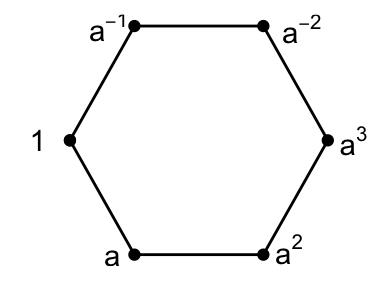
\includegraphics{t-algebra_files/figure-latex/unnamed-chunk-1-1} \end{center}

\end{example}

Set \(n = |X|\), the order of \(\Gamma\).

Pick a field \(K\) (\(=\mathbb{R}\) or \(\mathbb{C}\)). Then \(\mathrm{Mat}_X(K)\) denotes the \(K\) algebra of all \(n\times n\) matrices with entries in \(K\). (rows and columns are indexed by \(X\))

\emph{Adjacency matrix} \(A\in \mathrm{Mat}_X(K)\) is defined by
\begin{align}
A_{xy} & = \left\{\begin{array}{cl} 1 & \textrm{ if } \; xy\in E\\
0 & \textrm{ else } . \end{array}\right.
\end{align}

\begin{example}
Let \(a, b, c, d\) be labels of rows and columns. Then
\[A = \begin{matrix} \\ a\\ b\\c\\d\end{matrix}\begin{matrix}\begin{matrix} a & b & c & d \end{matrix}\\\begin{pmatrix} 0 & 1 & 1 & 0 \\ 1 & 0 & 1 & 1 \\
1 & 1 & 0 & 0 \\ 0 & 1 & 0 & 0 \end{pmatrix}\end{matrix}\]
\end{example}

The subalgebra \(M\) of \(\mathrm{Mat}_X(K)\) generated by \(A\) is called the \emph{Bose-Mesner algebra} of \(\Gamma\).

Set \(V = K^n\), the set of \(n\)-dimensional column vectors, the coorinates are indexed by \(X\).

Let \(\langle\; , \;\rangle\) denote the Hermitean inner product:
\[\langle u, v\rangle = u^\top\cdot v \quad (u, v\in V)\]
\(V\) with \(\langle\; , \;\rangle\) is the \emph{standard module} of \(\Gamma\).

\(M\) acts on \(V\): For every \(x\in X\), write
\[\hat{x} = \begin{pmatrix} 0 \\ \vdots \\ 0 \\ 1 \\ 0 \\ \vdots \\ 0 \end{pmatrix}\]
where \(1\) is at the \(x\) position.

Then
\[A\hat{x} = \sum_{y\in X, xy\in E}\hat{y}.\]
Since \(A\) is a real symmetrix matrix,
\[V = V_0 + V_1 + \cdots + V_r \quad \textrm{ some } r\in \mathbb{Z}^{\geq0},\]
the orthogonal direct sum of maximal \(A\)-eigenspaces.

Let \(E_i\in\mathrm{Mat}_X(K)\) denote the orthogonal projection,
\[E_i: V \longrightarrow V_i.\]
Then \(E_0, \ldots, E_r\) are the primitive idempotents of \(M\).
\[M = \mathrm{Span}_K(E_0, \ldots, E_r),\]
\[E_iE_j = \delta_{ij}E_i \quad \textrm{for all }\; i, j, \quad E_0 + \cdots + E_r = I.\]
Let \(\theta_i\) denote the eigenvalue of \(A\) for \(V_i\) in \(\mathbb{R}\). Without loss of generality we may assume that
\[\theta_0 > \theta_1 > \cdots > \theta_r.\]
Let
\[m_i = \textrm{the multiplicity of }\: \theta_i = \mathrm{dim} V_i = \mathrm{rank} E_i.\]
Set
\[\mathrm{Spec}(\Gamma) = \begin{pmatrix} \theta_0, & \theta_1, & \cdots, & \theta_r\\m_0, & m_1, & \cdots, & m_r\end{pmatrix}.\]
\textbf{Problem. }
What can we say about \(\Gamma\) when \(\mathrm{Spec}(\Gamma)\) is given?

The following Lemma\ref{lem:largestev}, is an example of Problem.

For every \(x\in X\),
\[k(x) \equiv \textrm{ valency of }x \equiv \textrm{ degree of }x \equiv |\{y\mid y\in X, \: xy\in E\}|.\]

\begin{definition}
\protect\hypertarget{def:regular}{}\label{def:regular}The graph \(\Gamma\) is regular\index{regular} of valency\index{valency} \(k\) if \(k = k(x)\) for every \(x\in X\).
\end{definition}

\begin{lemma}
\protect\hypertarget{lem:largestev}{}\label{lem:largestev}

With the above notation,

\((i)\) \(\theta_0\leq \max\{k(x) \mid x\in X\} = k^{\max}\).\\
\((ii)\) If \(\Gamma\) is regular of valency \(k\), then \(\theta_0 = k\).

\end{lemma}

\begin{proof}

\((i)\) Without loss of generality we may assume that \(\theta_0>0\), else done. Let \(v:=\sum_{x\in X}\alpha_x\hat{x}\) denote the eivenvector for \(\theta_0\).

Pick \(x\in X\) with \(|\alpha_x|\) maximal. Then \(|\alpha_x|\neq 0\).

Since \(Av = \theta_0v\),
\[\theta_0\alpha_x = \sum_{y\in X, xy\in E}\alpha_y.\]
So,
\[\theta_0 |\alpha_x| = |\theta_0\alpha_x| \leq \sum_{y\in X, xy\in E}|\alpha_y| \leq k(x)|\alpha_x| \leq k^{\max}|\alpha_x|.\]

\((ii)\) All 1's vector \(v = \sum_{x\in X}\hat{x}\) satisfies \(Av = kv\).

\end{proof}

\textbf{Subconstituent Algebra}

Let \(x, y\in X\) and \(\ell \in \mathbb{Z}^{\geq 0}\).

\begin{definition}
A path\index{path} of length \(\ell\) connecting \(x, y\) is a sequence
\[x = x_0, x_1, \ldots, x_{\ell} = y, \quad x_i\in X, \; 0\leq i\leq \ell\]
such that \(x_ix_{i+1}\in E\) for \(0\leq i \leq \ell-1\).
\end{definition}

\begin{definition}
The distance\index{distance} \(\partial(x,y)\) is the length of a shortest path connecting \(x\) and \(y\).
\[\partial(x,y) \in \mathbb{Z}^{\geq 0} \cup \{\infty\}.\]
\end{definition}

\begin{definition}
The graph \(\Gamma\) is connected\index{connected} if and only if \(\partial(x,y) < \infty\) for all \(x, y\in X\).
\end{definition}

From now on, assume that \(\Gamma\) is connected with \(|X|\geq 2\).

Set
\[d_\Gamma = d = \max\{\partial(x,y)\mid x, y\in X\} \equiv \textrm{the diameter of }\Gamma.\]
Fix a `base' vertex \(x\in X\).

\begin{definition}
\index{distance}
\[d(x) = \textrm{the diameter with respect to }x = \max\{\partial(x,y)\mid y\in X\} \leq d.\]
\end{definition}

Observe that
\[V = V_0^* + V_1^* + \cdots + V_{d(x)}^* \quad \textrm{(orthogonal direct sum)},\]
where
\[V_i^* = \mathrm{Span}_K(\hat{y}\mid \partial(x,y) = i) \equiv V_i*(x)\]
and \(V_i^* = V_i^*(x)\) is called the \(i\)-the subconstituent with respect to \(x\).

Let \(E_i^* = E_i^*(x)\) denote the orthogonal projection
\[E_i^*: V \longrightarrow V_i^*(x).\]
View \(E_i^*(x) \in \mathrm{Mat}_X(K)\). So, \(E_i^*(x)\) is diagonal with \(yy\) entry
\[(E_i^*(x))_{yy} = \begin{cases} 1 & \textrm{if } \: \partial(x,y) = i\\ 0 & \textrm{else,}\end{cases} \quad \textrm{ for } y\in X.\]
Set
\[M^* = M^*(x) \equiv \textrm{Span}_K(E_0^*(x), \ldots, E_{d(x)}^*(x)).\]
Then \(M^*(x)\) is a commutative subalgebra of \(\mathrm{Mat}_X(K)\) and is calle the \emph{dual Bose-Mesner algbara with respect to \(x\)}.

\begin{definition}[Subconstituent Algebra]
Let \(\Gamma = (X, E)\), \(x\), \(M\), \(M^*(x)\) be as above. Let \(T = T(x)\) denote the subalgebra of \(\mathrm{Mat}_X(K)\) generated by \(M\) and \(M^*(x)\). \(T\) is the \emph{subconstituent algebra}\index{subconstituent algebra} of \(\Gamma\) with respect to \(x\).
\end{definition}

\begin{definition}
A \(T\)-module \index{module} is any subspace \(W\subset V\) such that \(aw\in W\) for all \(a\in T\) and \(w\in W\).

\(T\)-module \(W\) is \emph{irreducible} if and only if \(W\neq 0\) and \(W\) does not properly contain a nonzero \(T\)-module.
\end{definition}

For any \(a\in \mathrm{Mat}_X(K)\), let \(a^*\) denbote the conjugate transpose of \(a\).

Observe that
\[\langle au, v\rangle = \langle u, a^*v\rangle \quad \textrm{for all }\; a\in \mathrm{Mat}_X(K), \textrm{ and for all } \; u,v\in V.\]

\begin{lemma}

Let \(\Gamma = (X,E)\), \(x\in X\) and \(T \equiv T(x)\) be as above.

\((i)\) If \(a\in T\), then \(a^*\in T\).

\((ii)\) For any \(T\)-module \(W\subset V\),

\[W^\bot := \{v\in V\mid \langle w, v\rangle = 0, \textrm{ for all }w\in W\}\]
is a \(T\)-module.

\((iii)\) \(V\) decomposes as an orthogonal direct sum of irreducible \(T\)-modules.

\end{lemma}

\begin{proof}

\((i)\) It is becase \(T\) is generated by symmetric real matrices

\[A, E^*_0(x), E^*_1(x), \ldots, E^*_{d(x)(x)}.\]

\((ii)\) Pick \(v\in W^\bot\) and \(a\in T\), it suffices to show that \(av\in W^\bot\). For all \(w\in W\),

\[\langle w, av\rangle = \langle a^*w, v\rangle = 0\]
as \(a^*\in T\).

\((iii)\) This is proved by the induction on the dimension of \(T\)-modules. If \(W\) is an irreducible \(T\)-module of \(V\), then

\[V = W + W^\bot \quad \textrm{(orthogonal direct sum)}.\]

\end{proof}

\textbf{Problem. }
What does the structure of the \(T(x)\)-module tell us about \(\Gamma\)?

Study those \(\Gamma\) whose modules take `simple' form. The \(\Gamma\)'s involved are highly regular.

\begin{remark}

\begin{enumerate}
\def\labelenumi{\arabic{enumi}.}
\tightlist
\item
  The subconstituent algebra \(T\) is semisimple as the left regular representation of \(T\) is completely reducible. See Curtis-Reiner 25.2 \citep{cr}.
\item
  The inner product \(\langle a, b\rangle_T = \mathrm{tr}(a^\top\bar{b})\) is nondegenerate on \(T\).
\item
  In general,
  \begin{align*}
  T\textrm{: Semisimple and Artinian} & \Leftrightarrow T\textrm{: Artinian with } J(T) = 0 \\
  & \Leftarrow T\textrm{: Artinian with nonzero nilpotent element} \\
  & \Leftarrow T \subset \mathrm{Mat}_X(K) \textrm{ such that for all } a\in T \textrm{ is normal.}
  \end{align*}
\end{enumerate}

\end{remark}

\hypertarget{lec2}{%
\chapter{Perron-Frobenius Theorem}\label{lec2}}

\textbf{Friday, January 22, 1993}

In this lecture we use the Perron Frobenius theory of nonnegative matrices to obtain informaiton on eigenvalues of a graph.

Let \(K = \mathbb{R}\). For \(n\in \mathbb{Z}^{> 0}\), pick a symmetrix matrix \(C\in \mathrm{Mat}_n(\mathbb{R})\).

\begin{definition}
The matrix \(C\) is \emph{reducible}\index{reducible} if and only if there is a bipartition \(\{1, 2, \ldots, n\} = X^+ \cup X^-\) (disjoint union of nonempty sets) such that \(C_{ij} = 0\) for all \(i\in X^+\), and for all \(j\in X^-\), and for all \(i\in X^-\), and for all \(j\in X^+\),i.e.,
\[ C \sim \begin{pmatrix} \ast & O \\ O & \ast \end{pmatrix}.\]
\end{definition}

\begin{definition}
The matrix \(C\) is \emph{bipartite}\index{bipartite} if and only if there is a bipartition \(\{1, 2, \ldots, n\} = X^+ \cup X^-\) (disjoint union of nonempty sets) such that \(C_{ij} = 0\) for all \(i,j\in X^+\), and for all \(i,j\in X^-\), i.e.,
\[ C \sim \begin{pmatrix} O & \ast \\ \ast  & O \end{pmatrix}.\]
\end{definition}

\textbf{Note.}

\begin{enumerate}
\def\labelenumi{\arabic{enumi}.}
\tightlist
\item
  If \(C\) is bipatite, for every eigenvalue \(\theta\) of \(C\), \(-\theta\) is an eigenvalue of \(C\) such that \(\mathrm{mult}(\theta) = \mathrm{mult}(-\theta)\).
\end{enumerate}

Indeed, let \(C = \begin{pmatrix} O & A \\ B & O \end{pmatrix}\),
\[\begin{pmatrix} O & A \\ B & O \end{pmatrix} \begin{pmatrix}x\\y\end{pmatrix} = \theta \begin{pmatrix}x\\y\end{pmatrix}\Leftrightarrow \begin{pmatrix} O & A \\ B & O \end{pmatrix} \begin{pmatrix}x\\-y\end{pmatrix} = -\theta \begin{pmatrix}x\\-y\end{pmatrix}, \]
where \(Ay = \theta x\) and \(Bx = \theta y\).

\begin{enumerate}
\def\labelenumi{\arabic{enumi}.}
\setcounter{enumi}{1}
\item
  If \(C\) is bipartite, \(C^2\) is reducible.
\item
  The matrix \(C\) is irreducible and \(C^2\) is reducible, if \(C_{ij} \geq 0\) for all \(i,j\) and \(C\) is reducible. (Exercise)
\end{enumerate}

\begin{remark}
Note 1. Even if \(C\) is not symmetric
\[\begin{pmatrix} O & A \\ B & O \end{pmatrix} \begin{pmatrix}x\\y\end{pmatrix} = \theta \begin{pmatrix}x\\y\end{pmatrix}\Leftrightarrow \begin{pmatrix} O & A \\ B & O \end{pmatrix} \begin{pmatrix}x\\-y\end{pmatrix} = -\theta \begin{pmatrix}x\\-y\end{pmatrix}\]
holds. So the geometrix multiplicities coincide. How about the algebraic multiplicities?

Note 3. Set \(x \sim y\) if and only if \(C_{xy}>0\). So the graph may have loops. Then
\[(C^2)_{xy} > 0 \Leftrightarrow \textrm{ if there exists } z\in X \textrm{ such that } x\sim z \sim y.\]
Note that \(C\) is irreducible if and only if \(\Gamma(C)\) is connected. Let
\begin{align}
X^+ & = \{y\mid \textrm{there is a path of even length from }x \textrm{ to }y\}\\
X^- & = \{y\mid \textrm{there is no path of even length from }x \textrm{ to }y\} \neq \emptyset.
\end{align}
If there is an edge \(y\sim z\) in \(X^+\) and \(w\in X^-\). Then there would be a path from \(x\) to \(y\) of even length.
So \(\mathrm{e}(X^+, X^+) = \mathrm{e}(X^-, X^-) = 0.\).
\end{remark}

\begin{theorem}[Perron-Frobenius]
\protect\hypertarget{thm:pf}{}\label{thm:pf}

Given a matrix \(C\) in \(\mathrm{Mat}_n(\mathbb{R})\) such that

\((a)\) \(C\) is symmetric.

\((b)\) \(C\) is irreducible.

\((c)\) \(C_{ij} \geq 0\) for all \(i,j\).

Let \(\theta_0\) be the maximal eigenvalue of \(C\) with eigenspace \(V_0 \subseteq \mathbb{R}^n\), and let \(\theta_r\) be the maximal eigenvalue of \(C\) with eigenspace \(V_r \subseteq \mathbb{R}^n\). Then the following hold.

\((i)\) Suppose \(0\neq v = \begin{pmatrix}\alpha_1\\\alpha_2\\\vdots\\\alpha_n\end{pmatrix} \in V_0\). Then \(\alpha_0 > 0\) for all \(i\), or \(\alpha_i < 0\) for all \(i\).

\((ii)\) \(\mathrm{dim}V_0 = 1\).

\((iii)\) \(\theta_r \geq -\theta_0\).

\((iv)\) \(\theta_r = \theta_0\) if and only if \(C\) is bipartite.

\end{theorem}

First, we prove the following lemma.

\begin{lemma}
\protect\hypertarget{lem:pfl}{}\label{lem:pfl}Let \(\langle \;,\; \rangle\) be the dot product in \(V = \mathbb{R}^n\). Pick a symmetric matrix \(B \in \mathrm{Mat}_n(\mathbb{R})\). Suppose all eigenvalues of \(B\) are nonnegative. (i.e., \(B\) is positive semidefinite.) Then there exist vectors \(v_1, v_2, \ldots, v_n\in V\) such that \(B_{ij} = \langle v_i, v_j\rangle\) for \((1\leq i, j \leq n)\).
\end{lemma}

\begin{proof}
By elementary linear algebra, there exists an orthonormal basis \(w_1, w_2, \ldots, w_n\) of \(V\) consisting of eigenvectors of \(B\). Set the \(i\)-th column of \(P\) is \(w_i\) and \(D = \mathrm{diag}(\theta_1,\ldots, \theta_n)\). Then \(P^\top P = I\) and \(BP = PD\).

Hence,
\[B = PDP^{-1} = PDP^\top = QQ^\top,\]
where
\[Q = P\cdot \mathrm{diag}(\sqrt{\theta_1}, \sqrt{\theta_2}, \ldots, \sqrt{\theta_n}) \in \mathrm{Mat}_n(\mathbb{R}).\]
Now, let \(v_i\) be the \(i\)-th column of \(Q^\top\). Then
\[B_{ij} = v_i^\top\cdot v_j^- = \langle v_i, v_j\rangle.\]
\end{proof}

Now we start the proof of Theorem \ref{thm:pf}.

\emph{Proof of Theorem \ref{thm:pf}}\((i)\)

Let \(\langle , \rangle\) denote the dot product on \(V = \mathbb{R}^n\). Set
\begin{align}
B & = \theta I - C\\
  & = \textrm{symmetric matrix with eigenvalues }\theta_0 - \theta_i \geq 0\\
  & = (\langle v_i, v_j\rangle)_{1\leq i,j\leq n}
\end{align}
with the same \(v_1, \ldots, v_n \in V\) by Lemma \ref{lem:pfl}.

Observe: \(\sum_{i = 1}^n \alpha_iv_i = 0\).

\emph{Pf.}
\begin{align}
\|\sum_{i = 1}^n \alpha_iv_i\|^2 & = \langle \sum_{i=1}^n\alpha_iv_i, \sum_{i=1}^n\alpha_iv_i\rangle\\
& = \begin{pmatrix} \alpha_1 &\ldots &\alpha_n\end{pmatrix}B\begin{pmatrix} \alpha_1\\\vdots\\\alpha_n\end{pmatrix}\\
& = v^\top Bv\\
& = 0,
\end{align}
since \(Bv = (\theta_0 I - C)v = 0\).

Now set
\[s = \textrm{the number of indices} i, \textrm{ where } \alpha_i >0.\]
Replacing \(v\) by \(-v\) if necessary, without loss of generality we may assume that \(s\geq 1\). We want to show \(s = n\).

Assume \(s < n\). Without loss of generality, we may assume that \(\alpha_i >0\) for \(1\leq s\leq s\) and \(\alpha_i = 0\) for \(s+1 \leq i \leq n\).
Set
\[ \rho = \alpha_1v_1 + \cdots + \alpha_sv_s = -\alpha_{s+1}v_{s+1} - \cdots - \alpha_nv_n.\]
Then, for \(i = 1,\ldots, s\),
\begin{align}
\langle v_i, \rho \rangle & = \sum_{j = s+1}^n -\alpha_j\langle v_i, v_j\rangle \quad (\langle v_i, v_j\rangle = B_{ij}, B = \theta_0I - C)\\
  & = \sum_{j = s+1}^n (-\alpha_{ij})(-C_{ij})\\
  & \leq 0.
\end{align}
Hence
\[0\leq \langle \rho, \rho\rangle = \sum_{i=1}^s \alpha_i \langle v_i, \rho\rangle \leq 0,\]
as \(\alpha > 0\) and \(\langle v_i, \rho\rangle \leq 0\). Thus, we have
\(\langle, \rho, \rho \rangle = 0\) and \(\rho = 0\).
For \(j = s+1, \ldots, n\),
\[0 = \langle \rho, v_j\rangle = \sum_{i=1}^s \alpha_i\langle v_i, v_j\rangle \leq 0,\]
as \(\langle v_i, v_j\rangle = -C_{ij}\).

Therefore,
\[0 = \langle v_i, v_j \rangle = -C_{ij} \textrm{ for } 1\leq i, \leq s, \: s+1 \leq j \leq n.\]
Since \(C\) is symmetric,
\[C = \begin{pmatrix} \ast & O \\ O & \ast\end{pmatrix}\]
Thus \(C\) is reducible, which is not the case. Hence \(s = n\).

\emph{Proof of Theorem \ref{thm:pf} \((ii)\).}

Suppose \(\dim V_0 \geq 2\). Then,
\[\dim\left(V_0 \cap \begin{pmatrix}1\\0\\\vdots\\0\end{pmatrix}^\bot\right) \geq 1.\]
So, there is a vector
\[0\neq v = \begin{pmatrix}\alpha_1\\\vdots\\\alpha_n\end{pmatrix} \in V_0\]
with \(\alpha_1 = 0\). This contradicts 1.

Now pick
\[0\neq w = \begin{pmatrix}\beta_1\\\vdots\\\beta_n\end{pmatrix} \in V_r.\]

\emph{Proof of Theorem \ref{thm:pf} \((iii)\).}

Suppose \(\theta_r < -\theta_0\). Since the eigenvalues of \(C^2\) are the squares of those of \(C\), \(\theta_r^2\) is the maximal eigenvalue of \(C^2\).

Also we have \(C^2w = \theta_r^2w\).

Observe that \(C^2\) is irreducible. (As otherwise, \(C\) is bipartite by Note 3, and we must have \(\theta_r = -\theta_0\).)
Therefore, \(\beta_i > 0\) for all \(i\) or \(\beta_i < 0\) for all \(i\). We have
\[\langle v, w\rangle = \sum_{i=1}^n\alpha_i\beta_j \neq 0.\]
This is a contradiction, as \(V_0 \bot V_r\).

\emph{Proof of Theorem \ref{thm:pf} \((iv)\)}

\(\Rightarrow\): Let \(\theta_r = -\theta_0\). Then \(\theta = \theta_1^2 = \theta_0^2\) is the maximal eigenvalue of \(C^2\), and \(v\) and \(w\) are linearly independent eigenvalues for \(\theta\) for \(C^2\). Hence, for \(C^2\), \(\mathrm{mult}(\theta) \geq 2\).

Thus by 2, \(C^2\) must be reducible. Therefore, \(C\) is bipartite by Note 3.

\(\Leftarrow\): This is Note 1.
\(\Box\)

Let \(\Gamma = (X, E)\) be any graph.

\begin{definition}
\(\Gamma\) is said to be \emph{bipartite}\index{bipartite} if the adjacency matrix \(A\) is bipartite. That is, \(X\) can be written as a disjoint union of \(X^+\) and \(X^-\) such that \(X^+, X^-\) contain no edges of \(\Gamma\).
\end{definition}

\begin{corollary}

For any (connected) graph \(\Gamma\) with
\[\mathrm{Spec}(\Gamma) = \begin{pmatrix}\theta_0 & \theta_1 &\cdots & \theta_r\\m_1 & m_1 & \cdots & m_r\end{pmatrix} \:\textrm{ with }\: \theta_0 > \theta_1 > \cdots > \theta_r.\]
Let \(V_i\) be the eigenspace of \(\theta_i\). Then the following holds.

\begin{enumerate}
\def\labelenumi{\arabic{enumi}.}
\item
  Supppose \(0\neq v = \begin{pmatrix} \alpha_1\\\vdots \\\alpha_n \end{pmatrix} \in V_0\in \mathbb{R}^n\). Then \(\alpha_i > 0\) for all \(i\) or \(\alpha_i < 0\) for all \(i\).
\item
  \(m_0 = 1\).
\item
  \(\theta_r \geq -\theta_0\) if and only if \(\Gamma\) is bipartite. In this case,
  \[-\theta_i = \theta_{r-i} \; \textrm{and} \; m_i = m_{r-i} \quad (0\leq i\leq r)\]
\end{enumerate}

\end{corollary}

\begin{proof}
This is a direct consequences of Theorem \ref{thm:pf} and Note 3.
\end{proof}

\hypertarget{lec3}{%
\chapter{Cayley Graphs}\label{lec3}}

\textbf{Monday, January 25, 1993}

Given graphs \(\Gamma = (X, E)\) and \(\Gamma' = (X', E')\).

\begin{definition}

A map \(\sigma: X \to X'\) is an \emph{isomorphism}\textbackslash index\{isomorophism of graphs whenever;

\begin{enumerate}
\def\labelenumi{\roman{enumi}.}
\tightlist
\item
  \(\sigma\) is one-to-one and onto,
\item
  \(xy\in E\) if and only if \(\sigma x \sigma y \in E'\) for all \(x, y\in X\).
\end{enumerate}

\end{definition}

We do not distinguish between isomorphic graphs.

\begin{definition}
Suppose \(\Gamma = \Gamma'\). Above isomorphism \(\sigma\) is called an \emph{automorphism}\index{automorphism} of \(\Gamma\). Then set \(\mathrm{Aut}(\Gamma)\) of all automorphisms of \(\Gamma\) becomes a finite group under composition.
\end{definition}

\begin{definition}
If \(\mathrm{Aut}(\Gamma)\) acts transitive on \(X\), \(\Gamma\) is called \emph{vertex transitive}\index{vertex transitive}.
\end{definition}

\begin{example}
A Cayley graphs:
\end{example}

\begin{definition}[Cayley Graphs]
\protect\hypertarget{def:cayley}{}\label{def:cayley}Let \(G\) be any finite group, and \(\Delta\) any generating set for \(G\) such that \(1_G \not\in \Delta\) and \(g\in \Delta \to g^{-1}\in \Delta\).
Then Cayley graph \(\Gamma = \Gamma(G, \Delta)\) is defined on the vetex set \(X = G\) with the edge set \(E\) define by the following. \index{Cayley graph}

\[E = \{(h_1,h_2)\mid h_1, h_2\in G, h_1^{-1}h_2\in \Delta\} = \{(h, hg) \mid h\in G, g\in \Delta\}\]
\end{definition}

\begin{example}

\(G = \langle a \mid a^6 = 1\rangle\), \(\Delta = \{a, a^{-1}\}\).

\begin{center}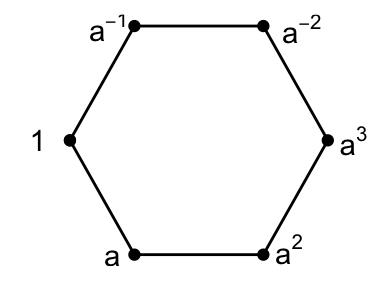
\includegraphics{t-algebra_files/figure-latex/unnamed-chunk-2-1} \end{center}

\end{example}

\begin{example}

\(G = \langle a \mid a^6 = 1\rangle\), \(\Delta = \{a, a^{-1}, a^2, a^{-2}\}\).

\begin{center}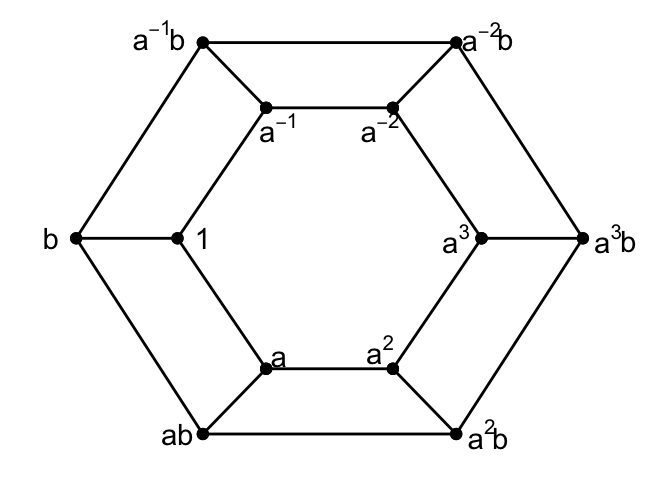
\includegraphics{t-algebra_files/figure-latex/unnamed-chunk-3-1} \end{center}

\end{example}

\begin{example}

\(G = \langle a, b \mid a^6 = 1, b^2, ab = ba\rangle\), \(\Delta = \{a, a^{-1}, b\}\).

\begin{center}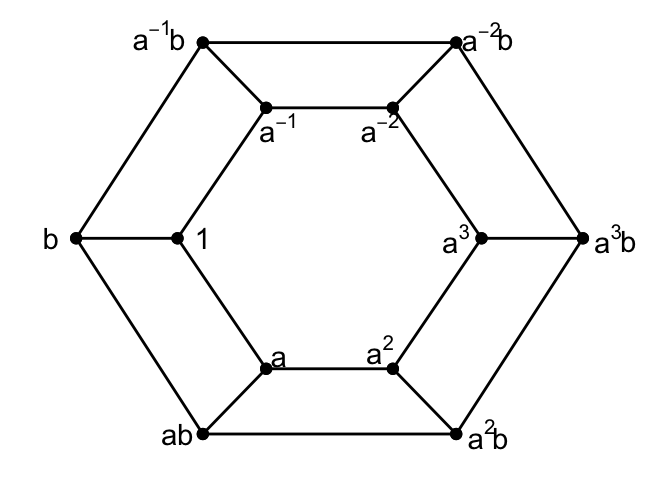
\includegraphics{t-algebra_files/figure-latex/unnamed-chunk-4-1} \end{center}

\end{example}

\begin{remark}
\(\mathrm{Aut}(\Gamma) \simeq D_6\times \mathbb{Z}_2\) contains two regular subgroups isomorphic to \(D_6\) and \(\mathbb{Z}_5 \times \mathbb{Z}_2\) and \(\Gamma\) is obtained as Cayley graphs in two ways.
\end{remark}

Cayley graphs are vertex transitive, indeed.

\begin{theorem}
The following hold.

\((i)\) For any Cayley graph \(\Gamma = \Gamma(G, \Delta)\), the map

\[G \to \mathrm{Aut}(\Gamma) \; (g\mapsto \hat{g})\]
is an injective homomorphism of groups, where
\[\hat{g}(x) = gx \quad \textrm{for all }\: g\in G \textrm{ and for all } x\in X (= G).\]
Also, the image \(\hat{G}\) is regular on \(X\). i.e., the image \(\hat{G}\) acts transitively on \(X\) with trivial vertex stabilizers.

\((ii)\) For any graph \(\Gamma = (X, E)\), suppose there exists a subgroup \(G \subseteq \mathrm{Aut}(\Gamma)\) that is regular on \(X\). Pick \(x\in X\), and let

\[\Delta = \{g\in G\mid \langle x, g(x)\in E\}.\]
Then \(1\not\in \Delta\), \(g\in \Delta \to g^{-1}\in \Delta\), and \(\Delta\) generates \(G\). Moreover, \(\Gamma \simeq \Gamma(G, \Delta)\).
\end{theorem}

\begin{proof}
\((i)\) Let \(g\in G\). We want to show that \(\hat{g}\in \mathrm{Aut}(\Gamma)\). Let \(h_1, h_2\in X = G\). Then,
\begin{align}
(h_1, h_2)\in E & \to h_1^{-1}h_2\in \Delta\\
  & \to (gh_1)^{-1}(gh_2)\in \Delta \\
  & \to (gh_1, gh_2)\in E\\
  & \to (\hat{g}(h_1), \hat{g}(h_2)) \in E.
\end{align}
Hence, \(\hat{g}\in \mathrm{Aut}(\Gamma)\).

Observe: \(g \mapsto \hat{g}\) is a homomorphism of groups:
\[\hat{1}_G = 1, \; \widehat{g_1g_2} = \widehat{g_1}\widehat{g_2}.\]

Observe: \(g \mapsto \hat{g}\) is one-to-one:
\[\widehat{g_1} = \widehat{g_2} \to g_1 = \widehat{g_1}(1_G) = \widehat{g_2}(1_G) = g_2.\]

Observe: \(\hat{G}\) is regular on \(X\): Clear by construction.

\((ii)\) \(1_G\not\in \Delta\): Since \(\Gamma\) has not loops, \((x, 1_Gx) \not\in E\).

\(g\in \Delta \to g^{-1}\in \Delta\):
\[g\in \Delta \to (x, g(x))\in E \to E \ni (g^{-1}(x), g^{-1}(g(x))) = (g^{-1}(x), x).\]

\(\Delta\) generates \(G\): Suppose \(\langle \Delta \subsetneq G\). Let \(\hat{X} = \{g(x)\mid g\in \langle \Delta\rangle\} \subsetneq X\). (\(\hat{X} \subsetneq X\) as \(G\) acts regularly on \(X\).)

Since \(\Gamma\) is connected, there exists \(y\in \hat{X}\) and \(z\in X\setminus \hat{X}\) with \(yz\in E\).

Let \(y = g(x)\), \(g\in \langle \Delta\rangle\), \(z\in h(x)\), \(h\in G\setminus \langle \Delta\rangle\). Then
\[(y,z)=(g(x),h(x))\in E \to (x,g^{-1}h(x))\in E \to g^{-1}h\in \langle \Delta \rangle \to h\in \langle \Delta \rangle. \]
This is a contradition. Therefore, \(\Delta\) generates \(G\).

Let \(\Gamma' = (X', E')\) denote \(\Gamma(G, \Delta)\). We shall show that
\[\theta: X' \to X \; (g\mapsto g(x))\]
is an isomorphism of graphs.

\(\theta\) is one-to-one: For \(h_1, h_2\in X' = G\),
\[\theta(h_1)=\theta(h_2) \to h_1(x) = h_2(x) \to h_2^{-1}h_1(x)=x \to h_2^{-1}h_1\in \mathrm{Stab}_G(x) = \{1_G\} \to h_1 = h_2.\]
(\(\mathrm{Stab}_G = \{g\in G\mid g(x) = x\}\).)

\(\theta\) is onto: Since \(G\) is transitive,
\[X = \{g(x)\mid g\in G\} = \theta(X') = \theta(G).\]

\(\theta\) respects adjacency: For \(h_1, h_2\in X' = G\),
\[(h_1,h_2)\in E' \leftrightarrow h_1^{-1}h_2\in \Delta \leftrightarrow (x, h_1^{-1}h_2(x))\in E \leftrightarrow (h_1(x),h_2(x))\in E \leftrightarrow (\theta(h_1), \theta(h_2))\in E.\]
Therefore \(\theta\) is an isomorphism between graphs \(\Gamma(G, \Delta)\) and \(\Gamma(X, E)\).
\end{proof}

How to compute the eigenvalues of the Cayley graph of and abelian group.

Let \(G\) be any finite abelian group. Let \(\mathbb{C}^*\) be the multiplicative group on \(\mathbb{C}\setminus \{0\}\).

\begin{definition}
A (linear) \(G\)-character\index{character} is any group homomorphism \(\theta: G \to \mathbb{C}^*\).
\end{definition}

\begin{example}
\(G = \langle a\mid a^3 =1\rangle\) has three characters, \(\theta_0, \theta_1, \theta_2\).
\[
\begin{array}{c|ccc}
\theta_i(a^j) & 1 & a & a^2 \\
\hline
\theta_0 & 1 & 1 & 1\\
\theta_1 & 1 & \omega & \omega^2\\
\theta_2 & 1 & \omega^2 & \omega
\end{array}, \quad \textrm{with }\; \omega = \frac{-1+\sqrt{-3}}{2}.
\]
Here \(\omega\) is a primitive cube root pf \(q\) in \(\mathbb{C}^*\), i.e., \(1+\omega + \omega^2 = 0\).
\end{example}

For arbitraty group \(G\), let \(X(G)\) be the set of all characters of \(G\).

Observe: For \(\theta_1, \theta_2\in X(G)\), one can define product \$\theta\_1\theta\_2:
\[\theta_1\theta_2(g) = \theta_1(g)\theta_2(g) \quad \textrm{for all }\; g\in G.\]
Then \(\theta_1\theta_2\in X(G)\).

Observe: \(X(G)\) with this product is an (abelian) group.

\begin{lemma}
\protect\hypertarget{lem:charactergroup}{}\label{lem:charactergroup}The groups \(G\) and \(X(G)\) are isomorphic for all finite abelian groups \(G\).
\end{lemma}

\begin{proof}
\(G\) is a direct sum of cyclic groups;
\[G = G_1\oplus G_2 \oplus \cdots \oplus G_m, \quad \textrm{where } \; G_i = \langle a_i\mid a_i^{d_i} = 1\rangle \quad (1\leq i\leq m).\]
Pick any alement \(\omega_i\) of order \(d_i\) in \(\mathbb{C}^*\), i.e., a primitive \(d_i\)-the root of \(1\). Define
\[\theta_i: G \to \mathbb{C}^* \quad (a_1^{\varepsilon_1}\cdots a_m^{\varepsilon_m} \mapsto \omega_i^{\varepsilon_i} \quad \textrm{where }\; 0\leq \varepsilon_i < d_i, 1\leq i\leq m).\]
Then \(\theta_i\in X(G)\). (Exercise)

Claim: There exists an isomorphism of groups \(G \to X(G)\) that sends \(a_i\) to \(\theta_i\).

Observe: \(\theta_i^{d_i} = 1\). For every \(g = a_1^{\varepsilon_1}\cdots a_m^{\varepsilon_m} \in G\),
\[\theta_i^{d_i}(g) = (\theta_i(g))^{d_i} = (\omega_i^{\varepsilon_i})^{d_i} = (\omega_i^{d_i})^{\varepsilon_i} = 1.\]
Observe: If \(\theta_1^{\varepsilon_1}\theta_2^{\varepsilon_2}\cdots \theta_m^{\varepsilon_m} = 1\) for some \(0\leq \varepsilon_i < d_i, 1\leq i\leq m\). Then \(\varepsilon_1 = \varepsilon_2 = \cdots = \varepsilon_m = 0\).

\emph{Pf.} \(1 = \theta_1^{\varepsilon_1}\theta_2^{\varepsilon_2}\cdots \theta_m^{\varepsilon_m}(a_i) = \omega_i^{\varepsilon_i}\), Since \(\omega_i\) is a primitive \(d_i\)-th root of \(1\), \(\varepsilon_i = 0\) for \(1\leq i\leq m\).

Observe: \(\theta_1, \ldots, \theta_m\) generate \(X(G)\). Pick \(\theta\in X(G)\). Since
\(a_i^{d_i} = 1\), \(1 = \theta(a_i^{d_i}) = \theta(a_i)^{d_i}\).

Hence \(\theta(a_i) = \omega^{\varepsilon_i}\) for some \(\varepsilon_i\) with \(0\leq \varepsilon_i < d_i\).

Now \(\theta = \theta_1^{\varepsilon_1}\cdots \theta_m^{\varepsilon_m}\), since these are both equal to \(\omega_i^{\varepsilon_i}\) at \(a_i\) for \(1\leq i \leq m\).

Therefore,
\[G \to X(G) \quad (a_i \mapsto \theta_i)\]
is an isomorphism of groups.
\end{proof}

\textbf{Note.} The correspondence above is clearly a group homomorphism.

\hypertarget{lec4}{%
\chapter{Examples}\label{lec4}}

\textbf{Wednesday, January 27, 1993}

\begin{theorem}
Given a Cayley graph \(\Gamma = \Gamma(G, \Delta)\). View the standard module \(V \equiv \mathbb{C}G\) (the group algebra), so
\[\left\langle \sum_{g\in G}\alpha_g g, \;\sum_{g\in G}\beta_g g\right\rangle = \sum_{g\in G}\alpha_g\overline{\beta_g}, \quad \textrm{with}\; \alpha_g, \beta_g\in \mathbb{C}.\]
For any \(\theta\in X(G)\), write
\[\hat{\theta} = \sum_{g\in G}\theta(g^{-1})g.\]
Then the following hold.

~~\((i)\) \(\langle \hat{\theta_1}, \hat{\theta_2}\rangle = |G|\) if \(\theta_1 = \theta_2\) and \(0\) othewise for \(\theta_1, \theta_2\in X(G)\). In particular, \(\{\hat{\theta}\mid \theta\in X(G)\}\) forms a basis for \(V\).

~~\((ii)\) \(A\hat{\theta} = \Delta_\theta \hat{\theta}\) for \(\theta \in X(G)\), where \(A\) is the adjacency matrix and

\[\Delta_\theta = \sum_{g\in \Delta}\theta(g).\]
In particular, the eigenvalues of \(\Gamma\) are precisely
\[\Delta_\theta \mid \theta\in X(G)\}.\]
\end{theorem}

\begin{proof}

\((i)\) Claim: For every \(\theta \in X(G)\), let

\[s:= \sum_{g\in G}\theta(g^{-1}) = \begin{cases} |G| & \text{if }\;\theta = 1\\
0 & \text{if } \;\theta \neq 1. 
\end{cases}\]
\emph{Pf.} Clear if \(\theta =1\).

Let \(\theta \neq 1\). Then \(\theta(h)\neq 1\) for some \(h\in G\).
\[s\cdot \theta(h) = \left(\sum_{g\in G}\theta(g^{-1})\right)\theta(h) = \sum_{g\in G}\theta(g^{-1}h) = \sum_{g'\in G}\theta(g'^{-1}) = s.\]
Since \(\theta(h)\neq 1\), \(s = 0\).

Claim. \(\theta(g^{-1}) = \overline{\theta(g)}\) for every \(\theta\in X(G)\) and every \(g\in G\).

Since \(\theta(g)\in \mathbb{C}\) is a root of \(1\),
\[|\theta(g)|^2 = \theta(g)\overline{\theta(g)} = 1.\]
On the other hand, since \(\theta\) is a homomorphism,
\[\theta(g)\theta(g^{-1}) = \theta(1) = 1.\]
Hence \(\theta(g^{1}) = \overline{\theta(g)}\).

Now
\begin{align}
\langle \widehat{\theta_1}, \widehat{\theta_2}\rangle & = \sum_{g\in G}\theta_1(g^{-1})\overline{\theta_2(g^{-1})}\\
& = \sum_{g\in G}\theta_1(g^{-1})\theta_2(g)\\
& = \sum_{g\in G}\theta_1\theta_2^{-1}(g^{-1})\\
& = \begin{cases} |G| & \text{if}\quad \theta_1\theta_2^{-1} = 1\\
0 & \text{if} \quad \theta_1\theta_2^{-1}\neq 1.
\end{cases}
\end{align}
Since \(|G| = |X(G)|\) by Lemma \ref{lem:charactergroup}, and \(\widehat{\theta_i}\)'s are orthogonal nonzero elements in \(V\), thet form a basis of \(V\).

~\((ii)\) Let \(\Delta = \{g_1, \ldots, g_r\}\). Then

\begin{align}
A\hat{\theta} & = A\left(\sum_{g\in G}\theta(g^{-1}g)\right)\\
& = \sum_{g\in G}\theta(g^{-1})(gg_1 + \cdots + gg_r) \quad (\Gamma(g) = \{gg_1, \ldots, gg_r\})\\
& = \sum_{i = 1}^r \left(\sum_{g\in G}\theta(g^{-1})(gg_i)\right)\\
& = \sum_{i=1}^r\left(\sum_{g\in G}\theta(g_ig_i^{-1}g^{-1})(gg_i)\right)\\
& = \sum_{i = 1}^r\left(\sum_{g\in G}\theta(g_i)\theta((gg_i)^{-1})gg_i\right)\\
& = \sum_{i = 1}^r\theta(g_i)\sum_{h\in G}\theta(h^{-1})h \\
& = \Delta_\theta\cdot \hat{\theta}.
\end{align}
Since \(\{\hat{\theta}\mid \theta\in X(G)\}\) forms a basis, the eigenvalues of \(\Gamma\) are precisely,
\[\{\Delta_\theta\mid \theta\in X(G)\}.\]

This completes the proof.

\end{proof}

\begin{example}
Let \(G = \langle a\mid a^6 = 1\rangle\), and \(\Delta = \{a, a^{-1}\}\). Pick a primitive 6-th root of 1, \(\omega\). Then
\[X(G) = \{\theta^i\mid 0\leq i\leq 5\} \quad \text{such that }\quad \theta(a) = \omega, \; \omega + \omega^{-1} = 1.\]

\begin{center}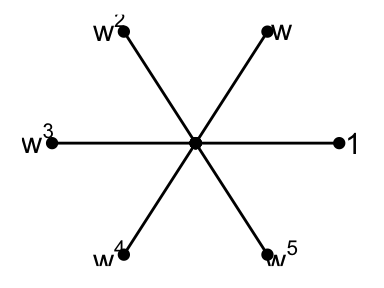
\includegraphics{t-algebra_files/figure-latex/unnamed-chunk-5-1} \end{center}

\[\begin{array}{c | c | c}
\varphi\in X(G) & \varphi(a) & \Delta_\varphi = \theta(a) + \theta(a)^{-1}\\
\hline
1 & 1 & 2\\
\theta & \omega & \omega+\omega^{-1} = 1\\
\theta^2 & \omega^2 & -1\\
\theta^3 & \omega^3 = -1 & -2\\
\theta^4 & \omega^4 & -1\\
\theta^5 & \omega^5 & 1
\end{array}\]
\[\text{Spec}(\Gamma) = \begin{pmatrix} 2 & 1 & -1 & -2\\ 1 & 2 & 2 & 1\end{pmatrix}.\]
\end{example}

\begin{example}
\(D\)-cube, \(H(D,2)\). Let
\[X = \{(a_1, \ldots, a_D)\mid a_i\in \{1,-1\}, \; 1\leq i\leq D\},\]
\[E = \{xy\mid x, y\in X, \; x, y \text{: different in exactly one coordinate}\}.\]
Also \(H(D,2)\) is a Cayley graph \(\Gamma(G, \Delta)\), where
\[G = G_1\oplus G_2 \oplus \cdots \oplus G_D, \]
\[G_i = \langle a_i\mid a_i^2  = 1\rangle,\quad \Delta = \{a_1, \ldots, a_D\}.\]
\end{example}

\textbf{Homework}: The spectrum of \(H(D,2)\) is
\[\begin{pmatrix} \theta_0 & \theta_1 & \cdots & \theta_D\\
m_0 & m_1 & \cdots & m_D\end{pmatrix},\]
where
\[\theta_i = D-2i \quad (0\leq i\leq D), \quad m_i = \binom{D}{i}.\]

\begin{remark}
Let \(\theta \in X(G)\). Then \(\theta: X \to \{\pm 1\}\). If
\[\nu(\theta) = |\{i\mid \theta(a_i) = -1\}|, \]
then \(\Delta_\theta = D-2i\). Since there are \(\binom{D}{i}\) such \(\theta\), we have te assertion.
\end{remark}

We want to compute the subconstituent algebra for \(H(D,2)\). First, we make a few observations about arbitrary graphd.

Let \(\Gamma = (X,E)\) be any graph, \(A\), the adjacemcy matrix of \(\Gamma\), and \(V\), the standard module over \(K = \mathbb{C}\).

Fix a base \(x\in X\). Write \(E_i^* = E_i^*(x)\), and
\[T \equiv T(x) = \text{the algebra generated by}\; A, E_0^*, E_1^*, \ldots .\]

\begin{definition}
Let \(W\) be any orreducible \(T\)-module (\(\subseteq V\)). Then the endpoint\index{endpoint} \(r \equiv r(W)\) satisfied
\[r = \min\{i\mid E_i^*W \neq 0\}.\]
The diameter\index{diameter} \(d = d(W)\) satisfied
\[d = |\{i\mid E_i^*W \neq 0\}| - 1.\]
\end{definition}

\begin{lemma}
\protect\hypertarget{lem:irreducible}{}\label{lem:irreducible}

With the above notation, let \(W\) be an irreducible \(T\)-module. Then

\((i)\) \(E_i^*AE_j^* = 0 \; \text{ if }\; |i-j|=1, \quad \neq 0 \; \text{ if }\; |i-j| = 1, \quad 0\leq i,j\leq d(x)\).\\
\((ii)\) \(AE_j^*W \subseteq E_{j-1}^*W + E_j^*W + E^*_{j+1}W\), \(0\leq j \leq d(x)\). \((E_i^*W = 0 \; \text{ if } i<j\) or \(i > d(x)\).)\\
\((iii)\) \(E^*_jW \neq 0\) if \(r\leq j \leq r+d\), \(=0\) if \(0\leq j\leq r\) or \(r+d < j \leq d(x)\).\\
\((iv)\) \(E_i^*AE^*_jW \neq 0\), if \(|i-j| = 1\) \((r \leq i,j \leq r+d)\).

\end{lemma}

\begin{proof}

\((i)\) Pick \(y\in X\) with \(\partial(x,y) = j\). We want to find \(E_i^*AE^*_j \hat{y}\). Note,

\[E_j^*\hat{y} = \begin{cases} 0 & \text{if }\; \partial(x.y)\neq j\\
\hat{y} & \text{if }\; \partial(x,y) = j.\end{cases}.\]
\begin{align}
E_i^*AE_j^*\hat{y} &= E_i^*A\hat{y} \\
& = E_i^*\sum_{z\in X, yz\in E}\hat{z}\\
& = \sum_{z\in X, yz\in E, \partial(x, z) = i}\hat{z} \qquad (*)\\
& = 0 \; \text{ if }\; |i-j|>1 \; \text{by triangle inequality.}
\end{align}
If \(|i-j| = 1\), there exist \(y, y'\in X\) such that \(\partial(x,y) = j\), \(\partial(x,y') = i\), \(yy'\in E\) by connectivity of \(\Gamma\). Hence
(*) contains \(\widehat{y'}\) and \(* \neq 0\).

\((ii)\) We have

\begin{align}
AE_j^*W & = \left(\sum_{i=0}^{d(x)}E_i^*\right)AE_j^*W\\
& = E_{j-1}^*AE^*_jW + E^*_jAE_j^*W + E^*_{j+1}AE_j^*W\\
& \subseteq E^*_{j-1}W + E^*_jW + E^*_{j+1}W.
\end{align}

\((iii)\) Suppose \(E_j^*W = 0\) for some \(j\) \((r\leq j \leq r+d)\). Then \(r < j\) by the definition of \(r\). Set

\[\tilde{W} = E^*_iW + E^*_{r+1}W + \cdots + E^*_{j-1}W.\]
Observe \(0\subsetneq \tilde{W} \subsetneq W\).
Also \(A\tilde{W} \subseteq \tilde{W}\) by \((ii)\) and \(E_i^*\tilde{W} \subseteq \tilde{W}\) for every \(i\) by construction.

Thus \(T\tilde{W} \subseteq \tilde{W}\), contradicting \(W\) beging irreducible.

\end{proof}

\hypertarget{lec5}{%
\chapter{\texorpdfstring{\(T\)-Modules of \(H(D,2)\), I}{T-Modules of H(D,2), I}}\label{lec5}}

\textbf{Friday, January 29, 1993}

Let \(\Gamma = (X, E)\) be a graph, \(A\) the adjacency matrix, and \(V\) the standard module over \(K = \mathbb{C}\).

Fix a base \(x\in X\) and write \(E_I^* \equiv E_i^*(x)\), and \(T \equiv T(x)\).

Let \(W\) be an irreducible \(T\)-module with endpoint \(r:= \min\{i\mid E_i^*W \neq 0\}\) and diameter \(d:=|\{i\mid E_i^*W\neq 0\}|-1\).

We have
\begin{align}
E_i^*W & \neq 0 & r\leq i \leq r+d\\
& = 0 & 0 \leq i < r \;\text{ or }\; r+d < i \leq d(x).
\end{align}

Claim: \(E_i^*AE_j^*W \neq 0\) if \$\i-j\textbar{} = 1 for \(r\leq i,j\leq r+d\). (See Lemma \ref{lem:irreducible}.)

Suppose \(E_{j+1}^*AE_j^*W = 0\) for some \(j\) with \(r \leq j < r+d\).

Observe that
\[\tilde{W} = E^*_rW + \cdot E^*_jW\]
is \(T\)-invariant with
\[0 \subsetneq \tilde{W} \subsetneq W.\]
Becase \(A\tilde{W} \subseteq \tilde{W}\) since \(AE_j^*W \subseteq E^*_{j-1}W + E^*_jW\),
\[E_k^*\tilde{W} \subseteq \tilde{W} \quad\text{for all }\; k,\]
we have \(T\tilde{W} \subseteq{W}\).

Suppose \(E_{i-1}^*AE_i^*W = 0\) for some \(i\) with \(r \leq i < r+d\).

Similarly,
\[\tilde{W} = E^*_iW + \cdot E^*_{r+d}.W\]
is a \(T\)-module with \(0\subsetneq \tilde{W} \subsetneq W\).

\begin{definition}
\protect\hypertarget{def:isomorphic-modules}{}\label{def:isomorphic-modules}Let \(\Gamma\), \(E^*_i\), and \(T\) be as above. Irreducible \(T\)-modules \(W\) and \(W'\) are isomorphic\index{isomorphic} whenever there is an isomorphism \(\sigma: W \to W'\) of vector spaces such that \(a\sigma = \sigma a\) for all \(a\in T\).
\end{definition}

Recall that the standard module \(V\) is an orthogonal direct sum of irreducible \(T\)-modules \(W_1 \oplus W_2 \oplus \cdots\). Given \(W\) in this list, the multiplicity\index{multiplicity} of \(W\) in \(V\) is
\[|\{j \mid W_j \simeq W\}|.\]

\begin{remark}
It is known that the multiplicity does not depend on the decomposition.
\end{remark}

Now assume that \(\Gamma\) is the \(D\)-cube, \(H(D,2)\) with \(D\geq 1\). Vew
\begin{align}
X & = \{a_1\cdots a_D\mid a_i\in \{1, -1\}, 1\leq i\leq D\},\\
E & = \{xy\mid x, y\in X, \; x, y \;\text{ differ in exactly 1 coordinate.}\}.
\end{align}
Find \(T\)-modules.

Claim: \(H(D,2)\) is bipartite with a partition \(X = X^+ \cup X^-\), where
\begin{align}
X^+ & = \{a_1\cdots a_D\in X\mid \prod a_i > 0\}\\
X^- & = \{a_1\cdots a_D \in X \mid \prod a_i < 0\}
\end{align}

Observe: for all \(y, z\in X\),
\[\partial(y,z) = i \Leftrightarrow y, z \; \text{ differ in exactly in }\; i\; \text{ coorinates with }\; 0\leq i\leq D.\]
Here, the diameter of \(H(D, 2) = D = d\) for all \(x\in X\).

\begin{theorem}
\protect\hypertarget{thm:hd2-modules}{}\label{thm:hd2-modules}Let \(\Gamma = H(D,2)\) be as above. Fix \(x\in X\), and write \(E_i^* = E^*_i(x)\), and \(T = T(x)\).

Let \(W\) be an irreducible \(T\)-module with endpoint \(r\), and diameter \(d\) with \(0\leq r \leq r+d\leq D\).

\((i)\) \(W\) has a basis \(w_0, w_1, \ldots, w_d\) with \(w_i\in E^*_{i+r}W\) for \(0\leq i\leq d\). With respect to which the matrix representing \(A\) is

\[
\begin{pmatrix}
0 & d & 0 & \cdots & 0 & 0 & 0\\
1 & 0 & d-1 & \cdots & 0 & 0 & 0\\
0 & 2 & 0 & \cdots & 0 & 0 & 0\\
0 & 0 & 3 & \cdots & 0 & 0 & 0\\
\cdots & \cdots & \cdots & \cdots & \cdots & \cdots & \cdots \\
0 & 0 & 0 & \cdots & 0 & 2 & 0\\
0 & 0 & 0 & \cdots & d-1 & 0 & 1\\
0 & 0 & 0 & \cdots & 0 & d & 0
\end{pmatrix}
\]

\((ii)\) \$ d= D - 2r\$. In particular, \(0\leq r\leq D/2\).

\((iii)\) Let \(W'\) denote an irreducible \(T\)-module with endpoint \(r'\). Then \(W\) and \(W'\) are isormorphic as \(T\)-modules if and only if \(r = r'\).

\((iv)\) The multiplicity of the irreducible \(T\)-module with endpoint \(r\) is

\[\binom{D}{r} - \binom{D}{r-1} \quad \text{if } 1\leq r \leq R/2,\]
and \(1\) if \(r = 0\).
\end{theorem}

\begin{proof}
Recall that \(\Gamma\) is vertex transitive. It is a Cayley graph.

Hence without loss of generality, we may assume that
\(x = \overbrace{11\cdots 1}^{D}\).

Notation: Set \(\Omega = \{1, 2, \ldots, D\}\). For every subset \(S \subseteq \Omega\), let
\[\hat{S} = a_1\cdot a_d \in X \quad a_i = \begin{cases} -1 & \text{if }\; i\in S\\ 1 & \text{if } i\not\in S.\end{cases}\]
In particular, \(\hat{emptyset} = x\) and
\[|S| = i \Leftrightarrow \partial(x, \hat{S}) = i \Leftrightarrow \hat{S}\in E^*_iV.\]
For all \(S, T\subseteq \Omega\), we say \(S\) covers T\$ if and only if \(S\supseteq T\) and \(|S| = |T| +1\).

Observe that \(\hat{S}, \hat{T}\) are adjacent in \(\Gamma\) if and only if either \(T\) coverse \(S\) or \(S\) coverr \(T\).

Define the `raising matrix'
\[R = \sum_{i=0}^D E^*_{i+1}AE^*_i.\]

Observe that
\[RE_i^*V \subseteq E^*_{i+1}V \; \text{ for }\; 0\leq i \leq D, \; \text{ and }E^*_{D+1}V = 0.\]
Indeed for any \(S\subseteq \Omega\) with \(|S| = i\),
\begin{align}
R\hat{S} & = RE^*_i\hat{S} \\
& = E^*_{i+1}A\hat{S} \\
& = \sum_{T_1 \subseteq \Omega, S \text{ covers }T_1} E^*_{i+1}\widehat{T_1} + \sum_{T \subseteq \Omega, T \text{ covers }S} E^*_{i+1}\hat{T}\\
& = \sum_{T \subseteq \Omega, T \text{ covers }S} E^*_{i+1}\hat{T}.
\end{align}

Define the `lowering matrix'
\[L = \sum_{i=0}^D E^*_{i-1}AE^*_i.\]

Observe that
\[LE_i^*V \subseteq E^*_{i-1V} \; \text{ for }\; 0\leq i \leq D, \; \text{ and }E^*_{-1}V = 0.\]
Indeed for any \(S\subseteq \Omega\),
\[L\hat{S} = \sum_{T\subseteq \Omega, S \text{ covers }T} \hat{T}.\]

Observe that \(A = L + R\).

For convenience, set
\[A^* = \sum_{i=0}^D (D-2i)E_i^*.\]

Claim: The following hold.

\((a)\) \(LR - RL = A^*\).\\
\((b)\) \(A*L - LA^* = 2L\).\\
\((c)\) \(A^*R - RA^* = -2R\).

In particular \(\mathrm{Span}(R,L, A^*)\) is a 'representation of Lie algebra \(\mathrm{sl}_2(\mathbb{C})\).

\begin{remark}[Lie Algebra sl2(C)]
\[\mathrm{sl}_2(\mathbb{C}) = \{X\mid \mathrm{Mat}(\mathbb{C} \mid \mathrm{tr}(X) = 0\}.\]
For \(X, Y\in \mathrm{sl}_2(\mathbb{C})\), define a binary operation \([X, Y] = XY - YX\).
\[A^*\sim \begin{pmatrix} 1 & 0 \\ 0 & -1\end{pmatrix}, \quad L\sim \begin{pmatrix} 0 & 1 \\ 0 & 0\end{pmatrix}, \quad R\sim \begin{pmatrix} 0 & 0 \\ 1 & 0\end{pmatrix}.\]
Then these satisfy the relations \((a)\) - \((c)\) above.
\end{remark}

\emph{Proof of Claim.}
Apply both sides to \(\hat{S}\) \quad \((S\subseteq \Omega)\). Say \(|S| = i\).

\emph{Proof of \((a)\):}
\begin{align} 
(LR - RL)\hat{S} & = L\left(\sum_{\substack{T \subseteq \Omega, T \text{ covers }S\\(D-i \text{ of them})}}\hat{T}\right) - R \left(\sum_{\substack{U \subseteq \Omega, S \text{ covers }U\\(i \text{ of them})}}\hat{T}\right)\\
& = (D-i)\hat{S} + \sum_{V \subseteq \Omega, |V| = i, |S\cap V| = i-1}\hat{V} - \left(i\hat{S} + \sum_{V \subseteq \Omega, |V| = i, |S\cap V| = i-1}\hat{V}\right)\\
& = (D-2i)\hat{S}\\
& = A^*\hat{S}.
\end{align}

\emph{Proof of \((b)\):}
\begin{align} 
(A^*L - LA^*)\hat{S} & = (D-2(i-1))L\hat{S} - (D-2i)L\hat{S} \quad (\text{since} \; L\hat{S}\in E^*_{i-1}V)\\
& = 2L\hat{S}.
\end{align}

\emph{Proof of \((c)\):}
\begin{align} 
(A^*R - RA^*)\hat{S} & = (D-2(i+1))R\hat{S} - (D-2i)R\hat{S} \quad (\text{since} \; R\hat{S}\in E^*_{i+1}V)\\
& = 2R\hat{S}.
\end{align}

Let \(W\) be an irreducible \(T\)-module with endpoint \(r\) and diameter \(d\) \((0\leq r \leq r+d \leq D)\).

\emph{Proof of \((i)\) and \((ii)\):}

Pick \(0\neq w \in E^*_rW\).

Claim: \(LRw = (D-2r)w\).

\emph{Pf.}
\begin{align} 
LRw & = (A^*+RL)w \quad (\text{by Claim }(a))\\
& = A^*w \quad (Lw \in E^*_{r-1}W = 0)\\
(D-2r)w.
\end{align}
Define
\[w_i = \frac{1}{i!}R^iw \in E^*_{r+i}W \quad (0\leq i \leq d).\]
Then,
\begin{align}
Rw_i & = (i+1)w_{i+1}\quad (0\leq i \leq d)\\
Rw_d & = 0 \quad (\text{by definition of }d)
\end{align}

Claim: \(Lw_0 = 0\) and
\[Lw_i = (D-2r-i+1)w_{i-1} \quad (1\leq i\leq d).\]

\emph{Pf.} We prove by induction on \(i\).
The case \(i=0\) is trivial, and the case \(i=1\) follows from above claim.
Let \(i\geq 2\),
\begin{align}
Lw_i & = \frac{1}{i}LRw_{i-1} = \frac{1}{i}(A^*+RL)w_{i-1} \quad (\text{by Claim (a)})\\
& \quad \text{(by induction hypothesis)}\\
& = \frac{1}{i}((D-2(r+i-1))w_{i-1} + (D-2r-(i-1)+1)Rw_{i-2} \quad (Rw_{i-2} = (i-1)w_{i-1})\\
& = \frac{1}{i}i(D-2r-i+1)w_{i-1}\\
& = (D-2r-i+1)w_{i-1}.
\end{align}

Claim: \(w_0, \ldots, w_d\) is a basis for \(W\).

\emph{Pf.}
Let \(W' = \mathrm{Span}\{w_0, \ldots, w_d\}\). Then \(W'\) is \(R\) and \(L\) invariant. So it is \(A = R+L\) invariant.

Also it is \(E^*_i\)-invariant for every \(i\).

Hence \(W'\) is a \(T\)-module.

Since \(W\) is irreducible, \(W' = W\).

As \(w_i\)'s are orthogonal, theyy are linearly independent. Note that \(w_i\neq 0\) by the definition of \(d\) and Lemma \ref{lem:irreducible} \((iv)\).

Claim: \(d = D-2r\).

\emph{Pf.}
By \((a)\),
\begin{align}
0 & = (LR - RL - A^*)w_d \\
& = 0 - (D-2r-d+1)Rw_{d-1} - (D-2(r+d))w_d\\
& = -d(D-2r-d+1)w_d - (D-2(r+d))w_d\\
& = (-dD + 2rd + d^2 - d - D + 2r + 2d)w_d\\
& = (d^2 + (2r-D+1)d + 2r - D)w_d\\
& = (d+2r-D)(d+1)w_d.
\end{align}
Hence \(d = D-2r\).

Therefore, with respect to a bais \(w_0, w_1, \ldots, w_d\),
\(A = L+R\), \(w_{-1} = w_{d+1} = 0\),
\[Lw_i = (d-i+1)w_{i-1}, \quad Rw_i = (i+1)w_{i+1}.\]
\[L = \begin{pmatrix} 0 & d & 0 & \cdots & 0 & 0\\
0 & 0 & d-1 & \cdots & 0 & 0\\
& & \cdots & \cdots & & \\
& & & & 0 & 1\\
0 & 0 & 0 & \cdots & 0 & 0
\end{pmatrix}, \qquad 
R = \begin{pmatrix} 0 & 0 & 0 & \cdots & 0 & 0\\
1 & 0 & 0 & \cdots & 0 & 0\\
0 & 2 & 0 & \cdots & & \\
& & & & 0 & 1\\
0 & 0 & 0 & \cdots & d & 0
\end{pmatrix}.\]
This completes the proof of \((i)\) and \((ii)\).
\end{proof}

\hypertarget{lec6}{%
\chapter{\texorpdfstring{\(T\)-Modules of \(H(D,2)\), II}{T-Modules of H(D,2), II}}\label{lec6}}

\textbf{Monday, February 1, 1993}

\textbf{Proof of Theorem \ref{thm:hd2-modules} Continued}

  \bibliography{book.bib,packages.bib}

\printindex

\end{document}
